\documentclass{article} % For LaTeX2e
\usepackage{nips14submit_e,times}
\usepackage{amsmath}
\usepackage{amsthm}
\usepackage{amssymb}
\usepackage{mathtools}
\usepackage{hyperref}
\usepackage{url}
\usepackage{algorithm}
\usepackage[noend]{algpseudocode}
%\documentstyle[nips14submit_09,times,art10]{article} % For LaTeX 2.09

\usepackage{bbm}
\usepackage{graphicx}
\usepackage{caption}
\usepackage{subcaption}
\usepackage{MnSymbol}

\def\eQb#1\eQe{\begin{eqnarray*}#1\end{eqnarray*}}
\def\eQnb#1\eQne{\begin{eqnarray}#1\end{eqnarray}}
\providecommand{\e}[1]{\ensuremath{\times 10^{#1}}}
\providecommand{\pb}[0]{\pagebreak}
\DeclarePairedDelimiter\ceil{\lceil}{\rceil}
\DeclarePairedDelimiter\floor{\lfloor}{\rfloor}

\newcommand{\E}{\mathrm{E}}
\newcommand{\Var}{\mathrm{Var}}
\newcommand{\Cov}{\mathrm{Cov}}

\def\Qb#1\Qe{\begin{question}#1\end{question}}
\def\Sb#1\Se{\begin{solution}#1\end{solution}}

\newenvironment{claim}[1]{\par\noindent\underline{Claim:}\space#1}{}
\newtheoremstyle{quest}{\topsep}{\topsep}{}{}{\bfseries}{}{ }{\thmname{#1}\thmnote{ #3}.}
\theoremstyle{quest}
\newtheorem*{definition}{Definition}
\newtheorem*{theorem}{Theorem}
\newtheorem*{lemma}{Lemma}
\newtheorem*{question}{Question}
\newtheorem*{preposition}{Preposition}
\newtheorem*{exercise}{Exercise}
\newtheorem*{challengeproblem}{Challenge Problem}
\newtheorem*{solution}{Solution}
\newtheorem*{remark}{Remark}
\usepackage{verbatimbox}
\usepackage{listings}
\usepackage{mathrsfs}
\title{ProbLimI: \\
Problem Set IV}


\author{
Youngduck Choi \\
CIMS \\
New York University\\
\texttt{yc1104@nyu.edu} \\
}


% The \author macro works with any number of authors. There are two commands
% used to separate the names and addresses of multiple authors: \And and \AND.
%
% Using \And between authors leaves it to \LaTeX{} to determine where to break
% the lines. Using \AND forces a linebreak at that point. So, if \LaTeX{}
% puts 3 of 4 authors names on the first line, and the last on the second
% line, try using \AND instead of \And before the third author name.

\newcommand{\fix}{\marginpar{FIX}}
\newcommand{\new}{\marginpar{NEW}}

\nipsfinalcopy % Uncomment for camera-ready version

\begin{document}


\maketitle

\begin{abstract}
This work contains solutions to the exercises of the problem set IV. The
chosen problems are 1,3, and 4.
\end{abstract}

\bigskip

\begin{question}[1]
\hfill
\begin{figure}[h!]
  \centering
    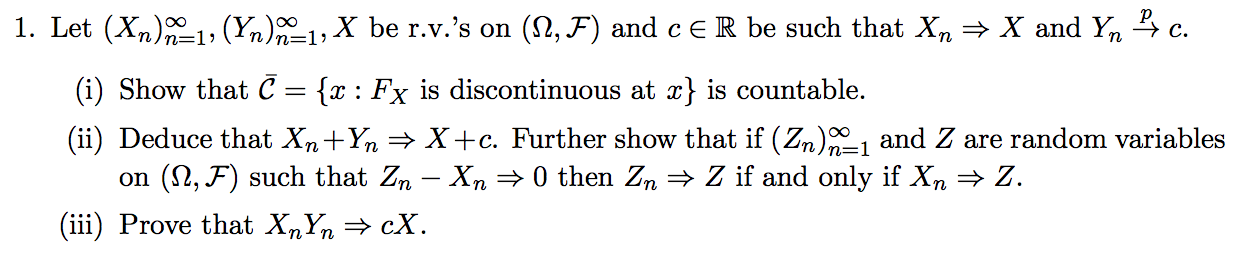
\includegraphics[width=0.7\textwidth]{problim-e4-p1.png}
\end{figure}
\end{question}
\begin{solution} \hfill \\
\textbf{(i)} We characterize the discontinuity points as  
\eQb
\overline{\mathscr{C}} &=& \bigcup_{n \in \mathbb{N}} 
\{x \in \mathbb{R} \> : \> 
\lim_{t \downarrow x} F_X(t) - F_X(x) \geq \dfrac{1}{n} \}
\eQe
Since $0 \leq F_X \leq 1$, it follows that 
\eQb
| \{x \in \mathbb{R} \> : \> 
\lim_{t \downarrow x} F_X(t) - F_X(x) \geq \dfrac{1}{n} \} | &\leq& n 
\eQe
for each $n \geq 1$. To see it explicitly, suppose otherwise, then there exists
some $n geq 1$ and 
$x,y \in \mathbb{R}$ such that $1 <\dfrac{n+1}{n} \leq F(x)-F(y)$, which is a 
contradiction. Therefore, $\overline{\mathscr{C}}$ is a countable union of
finite sets, so it is countable.

\bigskip

\textbf{(ii)}
Fix $\epsilon > 0$. Observe that
\eQb
\mathbb{P}(X_n + Y_n \leq a) &=& \mathbb{P}(X_n + Y_n \leq a , Y_n \geq c - \epsilon)
+ \mathbb{P}(X_n + Y_n \leq a , Y_n < c - \epsilon) \\
&\leq& \mathbb{P}(X_n \leq a - c + \epsilon) + \mathbb{P}(Y_n < c - \epsilon) \\
\eQe
and 
\eQb
\mathbb{P}(X_n + c \leq a - \epsilon) &\leq& \mathbb{P}(X_n + Y_n < a) + 
\mathbb{P}(Y_n \leq c - \epsilon) 
\eQe
for any $a \in \mathbb{R}$. As $Y_n \to_p c$ and $X_n$ converges in distribution to
$X$, by taking the limit with respect to $n$ on both inequalities above gives
\eQb
\limsup_{n} \mathbb{P}(X_n \leq a - c - \epsilon) &\leq&
\liminf_{n} F_{X_n + Y_n}(a) \leq \limsup_{n} F_{X_n + Y_n}(a) \leq 
\liminf_{n} \mathbb{P}(X_n < a -c + \epsilon)  
\eQe 
for any $a \in \mathbb{R}$. For $a$ that is a $F_{X+c}$ continuity point, we can 
take $\epsilon \to 0$, which gives 
\eQb
F_{X_n + Y_n}(a) \to \mathbb{P}(X + c \leq a)
\eQe
as $n \to \infty$.

\textbf{(iii)} Without loss of generality, assume that $c > 0$. Fix $0 < \delta < c$.
Observe that
\eQb
\mathbb{P}(X_n Y_n \leq a) &\leq& \mathbb{P}(X_n Y_n \leq a , |Y_n- c| \leq \delta)
+ \mathbb{P}(|Y_n - c| > \delta)
\eQe
for any $ a \in \mathbb{R}$ and $n \geq 1$. Using $Y_n \to_p c$,
we obtain
\eQb
\mathbb{P}(X_n Y_n \leq a) &\leq& \mathbb{P}(X_n \leq \dfrac{a}{c-\delta} + \delta
\eQe
for all large $n$. On the other hand,
\eQb
\mathbb{P}(X_n Y_n > a) &\leq& \mathbb{P}(X_n > \dfrac{a}{c+\delta}) + \delta.
\eQe 
Take $n \to \infty$ and $\delta \to 0$, we get the desired claim.
\hfill $\qed$

 
\end{solution}

\newpage

\begin{question}[2]
\hfill
\begin{figure}[h!]
  \centering
    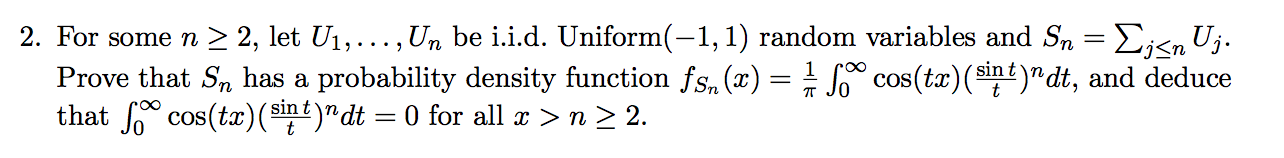
\includegraphics[width=0.7\textwidth]{problim-e4-p2.png}
\end{figure}
\end{question}
\begin{solution} \hfill \\
Fix $n \geq 1$.
Let $F_n$ be the cumulative distribution function of $S_n$. Then,
by independence, we obtain
\eQb
\phi_{S_n} &=& \phi_{U_1}^n = (\dfrac{\sin(t)}{t})^n.
\eQe
By Levy's inversion formula, it follows that
\eQb
F_n(b) - F_n(a) &=& \dfrac{1}{2\pi} \int_{-\infty}^{\infty} 
\dfrac{e^{-ita} - e^{itb}}{it} (\dfrac{\sin(t)}{t})^n dt 
\eQe
for $ a < b$ such that $a,b$ are continuity points of $F_{S_n}$.  
Now, observe that
the integrand on the RHS is continuous with respect to both $b,t$ variables
and the partial with respect to $b$ is also continuous with respect to $b,t$. Hence,
we can commute the partial with respect to $b$ with the integral to obtain
\eQb
f_n(b) &=& 
\int_{-\infty}^{\infty} 
\dfrac{\partial}{\partial b} 
(\dfrac{e^{-ita} - e^{itb}}{it} (\dfrac{\sin(t)}{t})^n) dt
= \dfrac{1}{2\pi} \int_{-\infty}^{\infty} e^{-itb}(\dfrac{\sin(t)}{t})^n dt \\ 
&=& \dfrac{1}{2\pi} \int_{-\infty}^{\infty} \cos(tb) (\dfrac{\sin(t)}{t})^n 
- i\sin(tb)(\dfrac{\sin(t)}{t})^n dt \\
&=& \dfrac{1}{2\pi} \int_{-\infty}^{\infty} \cos(tb) (\dfrac{\sin(t)}{t})^n dt
= \dfrac{1}{\pi} \int_{0}^{\infty} \cos(tb) (\dfrac{\sin(t)}{t})^n dt \\ 
\eQe 
for almost everywhere $b \in \mathbb{R}$, where the last two equalities follow
from considering evenness and oddness of the integrands and
the almost everywhere qualification comes from $(1-a)$. To conclude, we have
$S_n \leq n$ everywhere. If $f_{S_n}(x) > 0$ for some $x > n$, then by continuity of
$f_{S_n}$ on values larger than $n$, 
we can choose some small ball $B$ such that $B \cap (-\infty,n] = 
\emptyset$ and $\{w : S_n(w) \in B \} = \int_{B} f_{S_n}(x) dx > 0$, which 
contradictions $\{w : S_n(w) \leq n\} = 1$, and we are done. \hfill $\qed$ 

\end{solution}

\newpage

\begin{question}[3]
\hfill
\begin{figure}[h!]
  \centering
    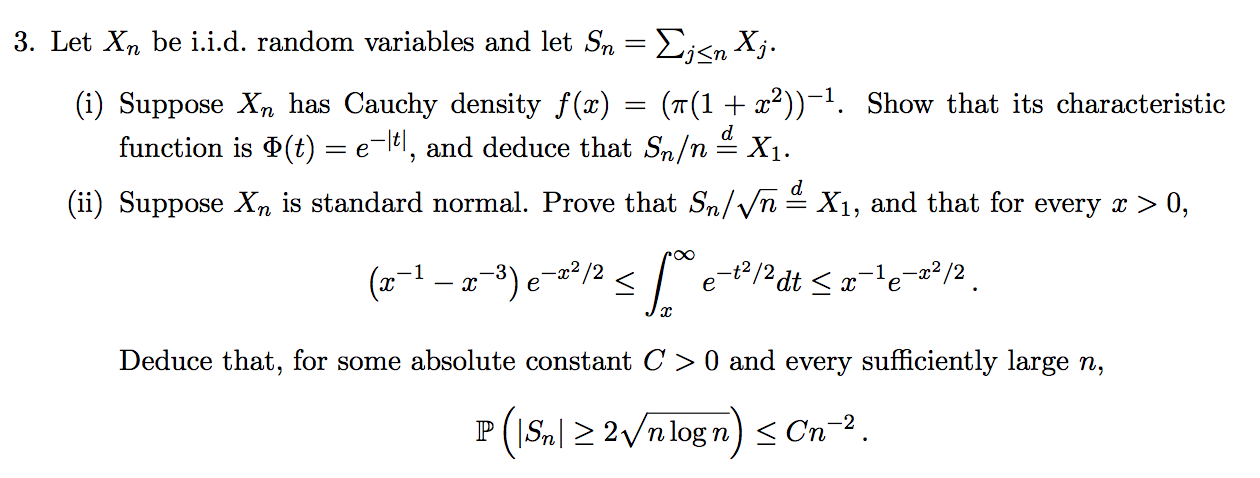
\includegraphics[width=0.7\textwidth]{problim-e4-p3.png}
\end{figure}
\end{question}
\begin{solution} \hfill \\
\textbf{(i)} Fix $t > 0$. We compute 
\eQb
\int_{\mathbb{R}} e^{itx}(\pi(1+x^2))^{-1} dx  
\eQe 
through Cauchy integral formula. Take the circle contour $\gamma_r$ 
in a counterclockwise orientation such that $L_z$ consists of the horizontal 
line from $-r$ to $r$ on the real axis and the $C_r$ the half circle contour
from $r$ to $-r$. Then, for sufficiently large $r$, by Cauchy residue theorem,
\eQb
e^{-t} &=& \int_{\gamma_r} \dfrac{e^{itz}}{\pi(1+z^2)} dz 
= \int_{-r}^{r} \dfrac{e^{itx}}{\pi(1+x^2)} dx + \int_{C_r} 
\dfrac{e^{itz}}{\pi(1+z^2)} 
\eQe 
because the residue can be computed as
\eQb
\lim_{z \to i} (z-i)\dfrac{e^{itz}}{\pi(1+z^2)} = \lim_{z \to i} 
\dfrac{e^{itz}}{\pi(z+i)} = \dfrac{e^{-t}}{2\pi i}.
\eQe
The result follows now, because as $r \to \infty$, by ML inequality,
the $C_r$ integral goes to $0$.

Now, for $ t < 0$, by a change of variable $u = -x$,
\eQb
\int_{\mathbb{R}} \dfrac{e^{itx}}{\pi(1 + x^2)} =
\int_{\mathbb{R}} \dfrac{e^{i(-t)x}}{\pi(1+u^2)} du = e^t. 
\eQe
Hence, this shows that $\phi(t) = e^{-|t|}$ for any $t \in \mathbb{R}$.
Using independence and ordinary properties of characteristic functions gives
\eQb
\Phi_{\frac{S_n}{n}}(t) &=& \prod_{i=1}^{n} \Phi_{\frac{X_i}{n}}(t) 
= \prod_{i=1}^{n} e^{-|\frac{t}{n}|} = e^{-|t|} \prod_{i=1}^{n} e^{-\frac{1}{n}} 
= e^{-|t|}
\eQe 
for any $t \in \mathbb{R}$. Therefore, by Fourier Uniqueness, we conclude that
$\dfrac{S_n}{n} = X_1$ in distribution as required. 


\bigskip

\textbf{(ii)} We have $\Phi_{X_1} = e^{-\frac{t^2}{2}}$. This fact is well known, and
if one wishes to derive it, the complex integration method works almost identically to 
the case above. Then, again by independence and properties of characteristic functions,
we compute
\eQb
\Phi_{\frac{S_n}{\sqrt{n}}} &=& \prod_{i=1}^{n} \Phi_{\frac{X_i}{\sqrt{n}}} 
= \prod_{i=1}^{n} e^{-\frac{t^2}{2n}} = e^{-t^2} \prod_{i=1}^{n} e^{-\frac{1}{2n}} 
= e^{-\frac{t^2}{2}} 
\eQe 
for any $t \in \mathbb{R}$. Therefore, by Fourier Uniqueness, it follows that
$\dfrac{S_n}{\sqrt{n}} = X_1$ in distribution.

\bigskip
We now show the first estimate. Fix $x > 0$. By integration by parts,
\eQb
\int_{x}^{\infty} e^{\frac{-t^2}{2}}dt &=& 
-\dfrac{1}{t}e^{-\frac{t^2}{2}}|_{x}^{\infty} - \int_{x}^{\infty} \dfrac{1}{t^2}
e^{-\frac{t^2}{2}} dt 
= \dfrac{1}{x}e^{-\frac{x^2}{2}} 
- \int_{x}^{\infty} \dfrac{1}{t^2}
e^{-\frac{t^2}{2}} dt 
\leq x^{-1}e^{\frac{-x^2}{2}}
\eQe
where the last inequality follows from the fact that
$\dfrac{1}{t^2}e^{-\frac{t^2}{2}}$ is a non-negative function on $\mathbb{R}$.
Now, again by integration by parts 
\eQb
\int_{x}^{\infty} e^{\frac{-t^2}{2}}
&=& x^{-1}e^{-\frac{x^2}{2}} - \int_{x}^{\infty} e^{-\frac{t^2}{2}} dt 
= (x^{-1} - x^{-3}) e^{-\frac{x^2}{2}} + C \int_{x}^{\infty} 
\dfrac{1}{t^4}e^{\frac{-t^2}{2}} dt 
\eQe 
for some positive constant $C$. Observe that the last integral is non-negative
as before. 
Combined with the above estimate, we finally obtain
\eQb
(x^{-1} - x^{-3}) e^{-\frac{x^2}{2}} &\leq& \int_{x}^{\infty} e^{-\frac{t^2}{2}}
dt  \leq  x^{-1}e^{\frac{-x^2}{2}}, 
\eQe
which completes the proof of the first estimate. Now, it follows that
\eQb
\mathbb{P}(\dfrac{|S_N|}{\sqrt{n}} \leq 2 \sqrt{\log(n)}) &\leq& 
2 ((2\sqrt{\log(n)})^{-1} e^{-2\log(n)}) \leq C \log(n)^{-\frac{1}{2}} n^{-2} 
\eQe 
for some positive constant $C$ and $n \geq 1$. Since $\log(n)^{-\frac{1}{2}}
n^{-2} = O(n^{-2})$, the result follows. \hfill $\qed$
\end{solution}

\newpage

\begin{question}[4]
\hfill
\begin{figure}[h!]
  \centering
    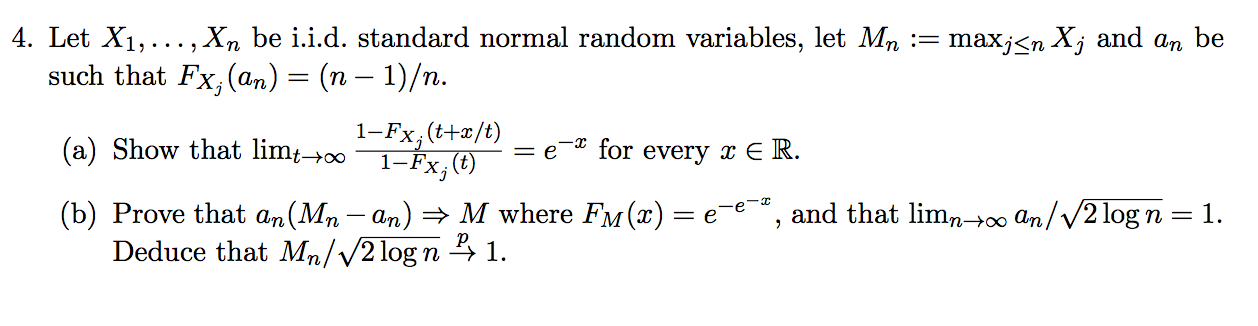
\includegraphics[width=0.7\textwidth]{problim-e4-p4.png}
\end{figure}
\end{question}
\begin{solution} \hfill \\
\end{solution}
\end{document}
